\documentclass[a4paper]{exam}
\newcommand{\Antwort}[1]{
	\fillin[#1]\hfill\qrcode{#1}\vspace{2em}
}
\usepackage{qrcode} % keine Umlaute verwende ä, ü, ö, 
\usepackage{listings}
\usepackage{tikz,pgfplots}

\title{
	Die drei grundlegenden Sprachen einer Webseite
	\newline
	Erfolgssicherung, Für die Dokumentation geeignet
	\begin{figure}[h!]
		\vspace{15mm}

		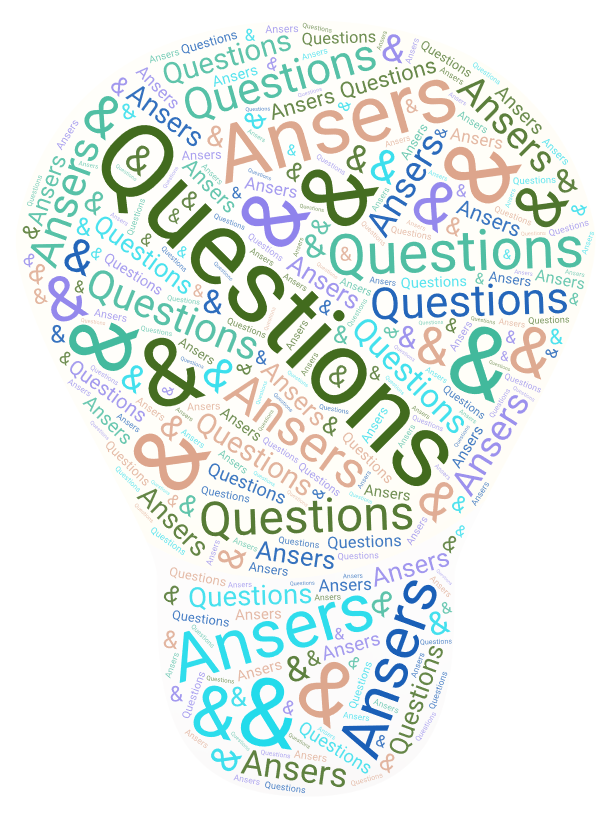
\includegraphics[scale=0.5]{../pics/lightBulpWordart.png}\centering
	\end{figure}
	\vfill
}
\author{Josef Sebastian Duschl}
\date{\today}


\begin{document}
	\maketitle
	\newpage
	\section{HTML}
		\begin{itemize}
			\item Was heißt HTML?
			\Antwort{Hypertext\ Markup\ Language,\ Kaskadierende Stilvorlagen}
			%\fillin[Hypertext Markup Language] \hfill\qrcode{Hypertext Markup %Language}\vspace{2em}
			
			\item Welche Art von Auszeichnungsprache ist es? %\fillin[texbasiert]\hfill\qrcode{textbasiert}\vspace{2em}\\
			\Antwort{textbasiert}
			
			\item Für was wird Sie verwendet?
			%\fillin[zur Strukturierung] \hfill \qrcode{zur Strukturierung}\vspace{2em}
			\Antwort{zur\ Strukturierung}
			
			\item Für welche Dokumente wird HTML verwendet?
			%\fillin[elektronische Dokumente] \hfill \qrcode{elektronische Dokumente}\vspace{2em}
			\Antwort{elektronische\ Dokumente}
			
			\item Was heißt WWW?
			%\fillin[World Wide Web] \hfill \qrcode{World Wide Web}\vspace{2em}
			\Antwort{World\ Wide\ Web}
			
			\item Gehört es zu den Grundlagen des WWW?
				\begin{oneparcheckboxes}
					\newline
					\choice yes
					\choice no
					\hfill\qrcode{yes\ }\vspace{2em}
				\end{oneparcheckboxes}

			\item Was ist ein Webbrowser?
			\Antwort{Ein\ Computerprogramm\ zur\ Darstellung\ einer\ Webseite}
			
			\item Welche zwei gängige Dokumentenarten lassen sich darstellen?\\
			\fillin[pdf] \fillin[html] \hfill \qrcode{pdf, html}\vspace{2em}
			
			\item Welche Aufgabe hat HTML?
			\Antwort{Text\ semantisch\ zu\ Strukturieren}
			
			\item Welche Matainformationen fallen Ihnen ein?
			\fillin[Sprache] \fillin[Autor] \hfill \qrcode{Sprache, Autor}
			
			\item Wer entwickelt HTML weiter?
			\fillin[W3C] \fillin[WHATWG] \hfill \qrcode{W3C, WHATWG}
			
			\item Wer hat Sie erfunden?
			\Antwort{Europaeischen\ Organisation\ fuer\ Kernforschung,\ CERN}
			
			\item Wann wurde Sie erfunden?
			\Antwort{1989}
			\item Finde den Fehler!
		\end{itemize}
		\begin{lstlisting}[language=html]
<html>
    <head>
        <title>Page Title</title>
    </head>
    <body>
    
        <h1>This is a Heading</h1>
        <p>This is a paragraph.</p>
        
    </body>
</html> 
		\end{lstlisting}
		\vfill
		\qrcode{https://www.w3schools.com/html/tryit.asp?filename=tryhtml_intro}
		\newpage
		
		\section{CSS}
			\begin{itemize}
				\item Was heißt CSS?
				\Antwort{Cascading Style Sheets, Kaskadierende Stilvorlagen} 
				
				\item Für Welche Art von Dokumenten ist die Sprache gedacht?
				\Antwort{Fuer\ elektronische\ Dokumente}
				
				\item Für Welche Erstellung ist Sie gedacht?
				\Antwort{Fuer\ Gestaltungsanweisungen}
				
				\item Wer hat Sie erfunden?
				\Antwort{Hakon\ Wium\ Lie, CERN}
				
				\item Wann wurde Sie erfunden?
				\Antwort{1996}
				
				\item In welchem Tag befindet Sie sich?
				\Antwort{<style>}
				\newpage
				\item Finde den Fehler!
			\end{itemize}

				\begin{lstlisting}
<!DOCTYPE html>
<html>
	<head>
		<style>
			body {
				background-color: lightblue;
			}

			h1 {
				color: white;
				text-align: center;
			}

			p {
				font-family: verdana;
				font-size: 20px;
			}
	</head>
	<body>

		<h1>My First CSS Example</h1>
		<p>This is a paragraph.</p>

	</body>
</html>
				\end{lstlisting}
				\vfill
\qrcode{https://www.w3schools.com/css/tryit.asp?filename=trycss_default}
				\newpage
				\section{JavaSript}
			\begin{itemize}
				\item Was für eine Sprache ist JavaScript?
				\Antwort{Eine\ Srcriptsprache}
				
				\item Für was wurde Sie ursprünglich entwickelt
				\Antwort{Um Benutzerinteraktionan\ auszuwerten}
				
				\item Was macht JavaScript mit Inhalten?
				\Antwort{Inhalte Veraendern,\ nachladen,\ generieren}
				
				\item Wieso nicht LiveScript?
				\Antwort{Um die Popularitaet\ von\ Java\ zu\ nutzen}
				
				\item welche Besonderheiten weißt Javascript in der Sprache noch auf?\\
				\Antwort{Sie\ ist\ objektorientiert,\ prozedural,\ funktional}
				\item Was ist ECMAScript?
				\Antwort{beschreibt\ den\ standardisierten\ Sprachkern\ von\ JavaScript}
				\item Was heißt ECMA?
				\Antwort{European\ Computer\ Manufacturers\ Association,\ Europaeischer\ Verband\ der\ Computerhersteller}
				\item Für was steht ECMA?
				\Antwort{dynamische\ typisierte,\ objektorienterte\ aber klassenlose\ Skripsprache}
				
				\item Wer hat Sie erfunden?
				\Antwort{Netscape\ \&\ Sun\ Microsystmes\ -> Oracle}
				
				\item Wann wurde Sie erfunden?
				\Antwort{1996}
				
				\item Mit welchem Tagnamen wird Javascript eingeleitet?
				\Antwort{<script>}
				
				\item Finde den Fehler
			\end{itemize}
				\begin{lstlisting}
<!DOCTYPE html>
<html>
	<head>
		<script>
			function myFunction() {
				document.getElementById().innerHTML 
					= "Paragraph changed.";
			}
		</script>
	</head>
	<body>
		<h2>JavaScript in Head</h2>
		<p id="demo">A Paragraph.</p>
		<button type="button" onclick="myFunction()">Try it</button>
	</body>
</html>
				\end{lstlisting}
				\vfill
				\qrcode{https://www.w3schools.com/js/tryit.asp?filename=tryjs_whereto_head}
\end{document}
